\section{Development Method and Organisational Tools}
The entire GIRAF project met to discuss the information gathered from last years reports, alongside pros and cons of the process they used.
Last year's reports recommended to change different aspects of their development process, and their advice has been taken into consideration.
This section will first present the chosen development method as has been chosen at this meeting, and will finally present the tools that will accommodate the development method.


\subsection{Development Method of the Multi--Project}\label{devmethod}
The previous semester of the GIRAF project used the agile development method \textit{Scrum of Scrum}, which is a scaled version of \textit{Scrum}.
This is also the choice for the multi--project of 2016, but where as last year they had three--layers of Scrum of Scrums, as the multi--project was separated into three further sub--projects:
\begin{itemize}
	\item Applications
	\item Database
	\item Build \& Deployment
\end{itemize}

This is changed for the multi--project of 2016, as many of the reports from last year recommended to change this, such that any group would be able to work on any tasks which occur during the project.

In order to explain how Scrum of Scrum works, a brief explanation of Scrum is now presented.
This is in turn also how we will be working internally in group SW618F16.

\subsubsection{Scrum}\label{scrum}

For the development of this project we want to use Scrum to gain the benefits that it can yield if used correctly.
In the book \textit{Agile Software Development with Scrum}\cite{scrumbookschwaber}~Ken Schwaber argues that Scrum:
\begin{displayquote}
(...)~\textit{enables people to work together effectively, and by doing so, it enables them to produce complex, sophisticated products.}
\end{displayquote}

Scrum makes progress visible and helps teams cut through the noise a project creates, and allows the teams to deal with smaller pieces of the problems instead.
If a problem is big and complex, Scrum allows the team to deal with it incrementally.
The nature of Scrum especially the daily Scrum meeting, which will be explained shortly, allows a team to share knowledge with each other, and discover problems with current assignments, which in turn makes the team more responsive to changes from these appearing problems because everyone is in agreement.
We want to use Scrum for this project because of the above mentioned reasons, but to sum it up, we want to use Scrum to create a structure and visible progress for a project where we keep getting new knowledge from the already existing codebase, and from the other 8 teams which we are working together with for the multi--project.

\newpage
We use parts of the version of Scrum as defined by Sommerville in his book, Software Engineering in \cite[Chapter~3]{SEBOOK}.
The parts used are presented here.

\begin{description}
	\item[Daily Scrum] \hfill \\
	Everyday we start out by having a daily Scrum, which is a meeting where each person in the group is asked the following questions:
		\begin{itemize}
		    \item What did you do yesterday?
			\item What will you do today?
			\item What obstacles are in your way or slowing you down?
		\end{itemize}
		This helps make sure that all group members know what each other are doing, while also giving an opportunity to ask for help if needed.
	\item[Sprints] \hfill \\
	A sprint is a working period where the group sets out to complete different tasks before the sprint end.
	The duration of the sprint is determined by the Scrum Master and Product Owner.
	\item[User Story] \hfill \\
	A user story is a formulation of a requirement.
	Each user story has been given a priority by the Product Owner, these are in descending order of priority: \pblocking, \phigh, \pnormal, \plow~and \pwish.
	Across the multi--project we have decided upon the format for a user story to be: \enquote{As a <type of user>, I want <some goal> so that <some reason>}.
	Each user story is estimated to take a period of time.
	\item[Task] \hfill \\
	A user story can be split into multiple tasks, as sometimes they can be broken down into separate issues.
	Each of these can be done by either the same person or different people.
	\item[User Story Estimation] \hfill \\
	Each user story has an estimated amount of effort it will take to complete it.
	We use the unit \textit{Effort Points} (\textbf{EP}) to evaluate each user story.
	Each sprint has a number of EP available; the sum of EP in the stories should be close to the number of EP available in the sprint, although slightly lower to account for time spent on reviewing other user stories and the report.
	We determine EP for user stories using a technique called Planning Poker.
	In Planning Poker, each member of the group selects the number of EP they think a given user story is worth, without the others knowing before everyone has selected a number of EP.
	If there is agreement then the user story is given that amount of EP.
	Otherwise each group member should tell the others why they think they have estimated correctly, and then the process starts over until an agreement is reached.
	\item[Product Backlog] \hfill \\
	A product backlog is a list of tasks which are to be done in order for the project to be complete.
	It replaces traditional requirements lists, and can develop throughout the development process by adding tasks.
	\item[Sprint Backlog] \hfill \\
	A sprint backlog contains the tasks chosen from the product backlog by the development team to be completed in the sprint.
	As task estimation is done after tasks have been chosen from the product backlog, the number of tasks for a given sprint might have been too many or too few, if this problem occurs then the group can, in collaboration with the product owner, choose to remove or add tasks during a sprint.
	\item[Scrum Master] \hfill \\
	The Scrum master is a role of one of the developers of the project, it is the Scrum masters job to make sure that the development team uses Scrum correctly, and also helps the product owner organising the product back-log.
	\item[Product Owner] \hfill \\
	The product owner is another role, which deals with understanding what the customer wants.
	The product owner is also in charge of the product backlog, prioritising the tasks and ensures that the tasks are understandable such that it is easy for a developer to proceed with the development of the task.
	The product owner priotises the tasks after \enquote{what they fell are the best for the project and the customers}.
	\item[Scrum Board] \hfill \\
	A Scrum board is a board which contains all tasks from the sprint-backlog.
	These tasks can have different sub-tasks, and these are then moved from different columns depending on where they are currently reside in development.
	They can be in five different columns:
	\begin{multicols}{5}
		\begin{itemize}
		\item Story
		\item To-do
		\item Doing
		\item Review
		\item Done
	\end{itemize}
	\end{multicols}

	\begin{figure}
	  \begin{center}
	    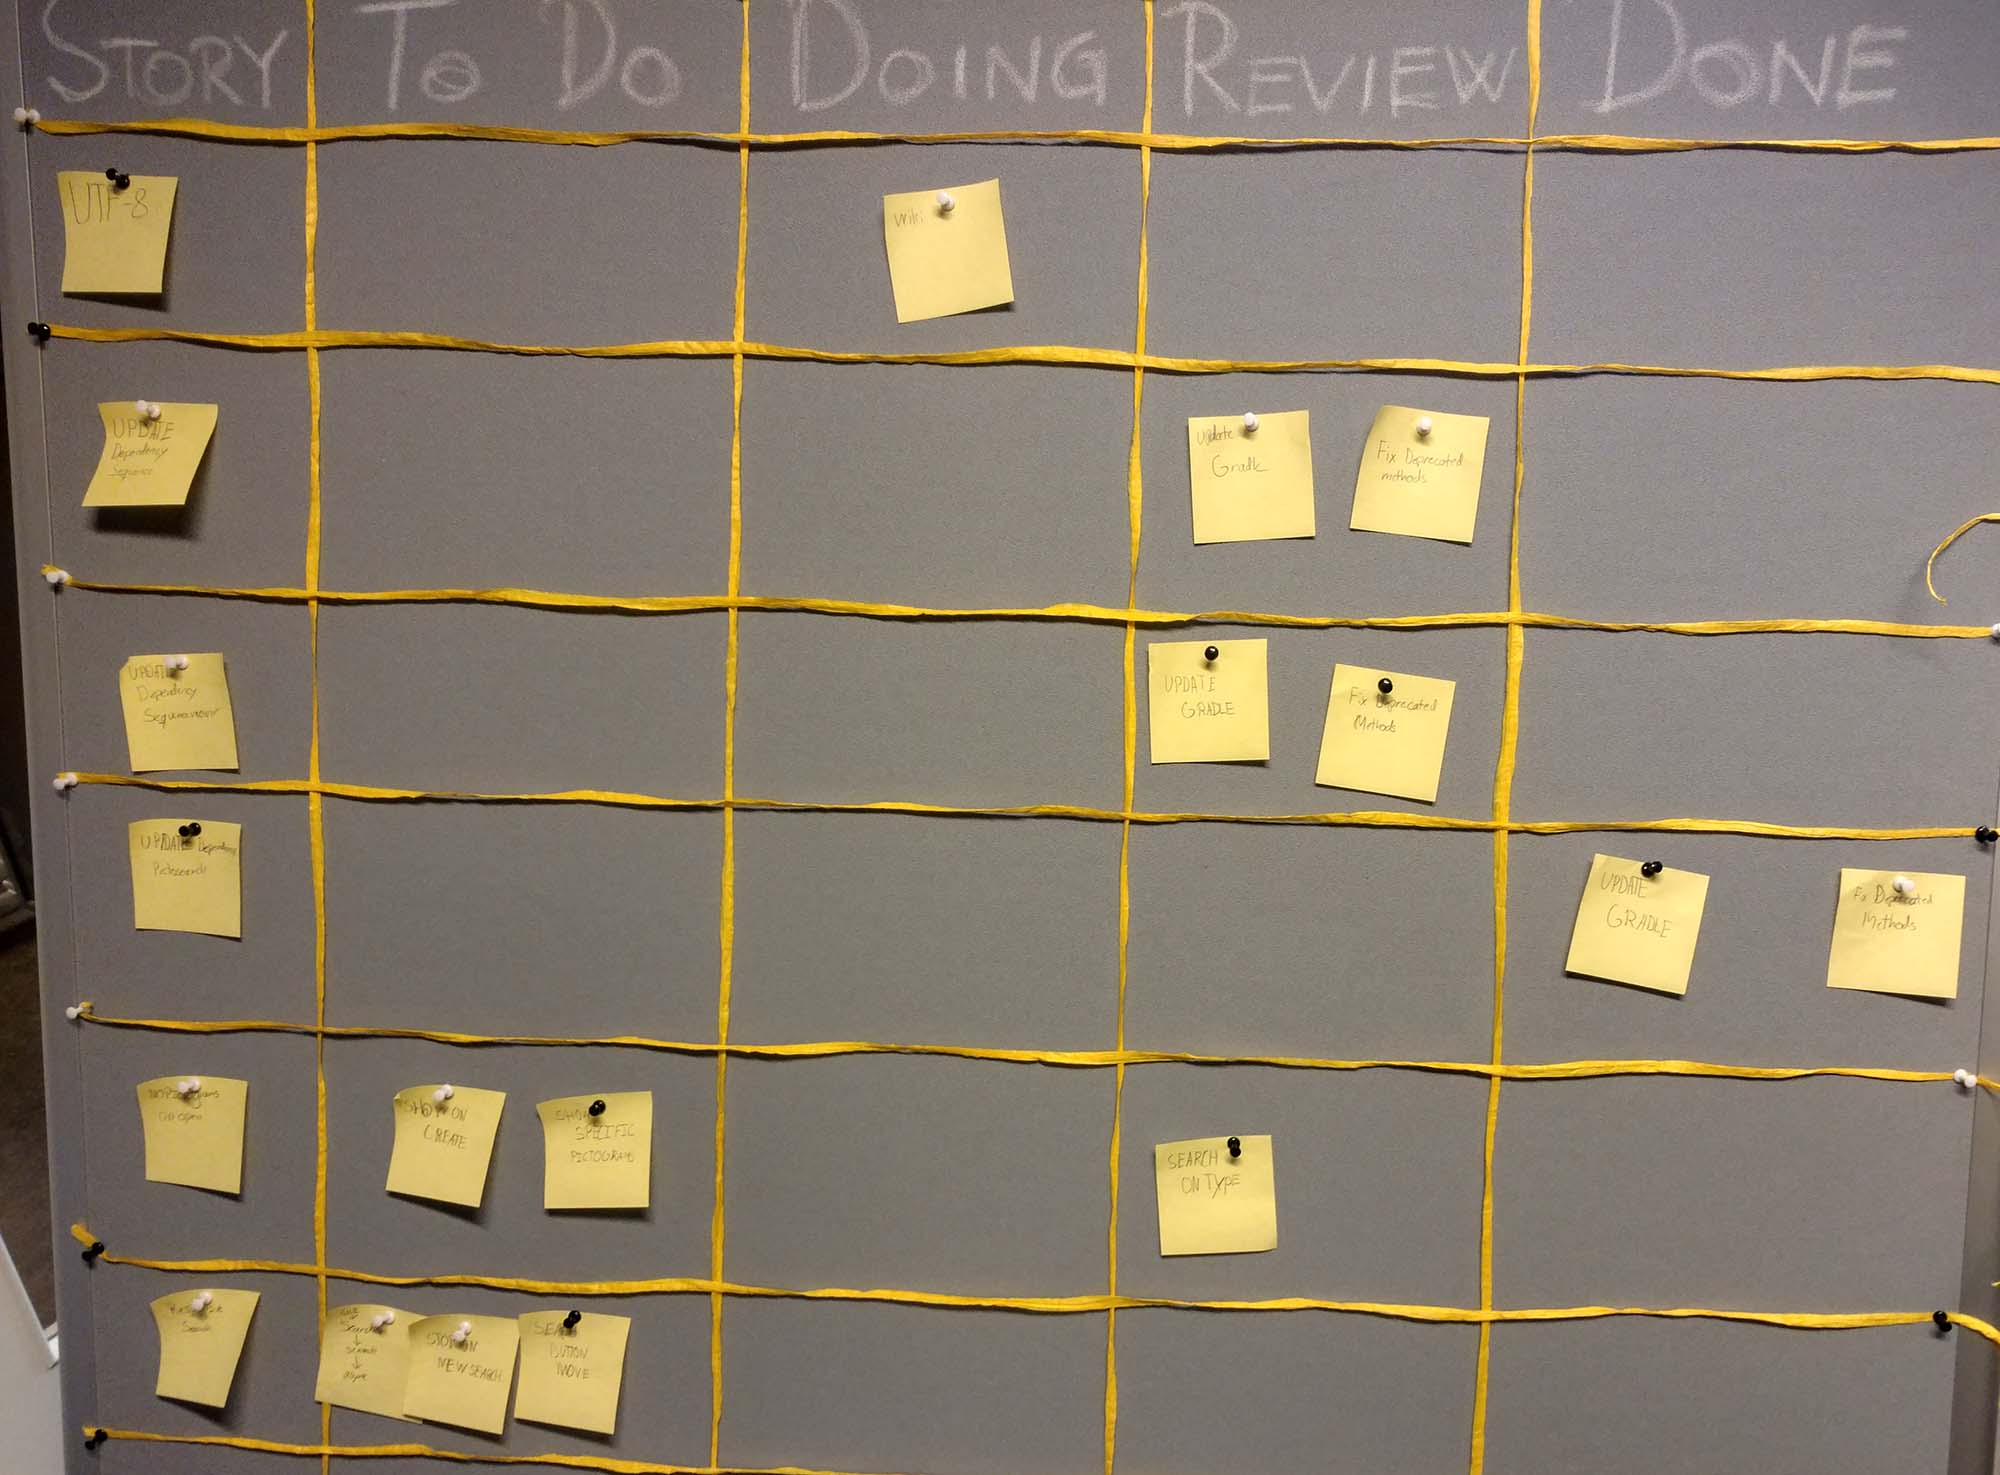
\includegraphics[width=0.80\textwidth]{figures/img/scrumboard_compressed.jpg}
	  \end{center}
	  \caption{Our Scrum Board.}
	  \label{fig:scrumboard}
	\end{figure}
	The Scrum board works well to make sure that progress is visible, and to show what different tasks are currently being worked on.
	A picture of our Scrum Board is shown in \myref{fig:scrumboard}.
\end{description}

\subsection{Pair Programming}\label{subsubsec:pairprogramming}
Pair programming is a technique in which two programmers develop software on the same computer.
For practical reasons only one of them uses the keyboard and mouse while the other person is there to discuss solutions, and help with making decisions.
While this method has been found to take more time overall (about 15~\% more) for developing a piece of software, it has also been found to increase the quality of code and the design.
It is also useful for learning purposes, since the pair will learn from each other.
Another advantage is that at least two people will have an understanding of the code produced.
Pair programming was first described by Don Wells for Extreme Programming\cite{pairAgile}, but has since spread to be used outside of Extreme Programming.
For more information about the benefits and costs of pair programming see \textit{The Costs and Benefits of Extreme Programming}\cite{cockburn2000costs} by Alistair Cockburn et al.

\subsubsection{Scrum of Scrum}
The Scrum of Scrum consists of multiple groups, all using Scrum, each group then has an ambassadors who meets with the other ambassadors for the Scrum meetings.
This is an adaptation of Craig Larman's description of Scrum of Scrums in the book \textit{Agile \& Iterative Development}\cite{ScrumBOOK}.
The structure of the Scrum of Scrum can be seen on \myref{fig:ScrumofScrum}

\begin{figure}[!htb]
\centering
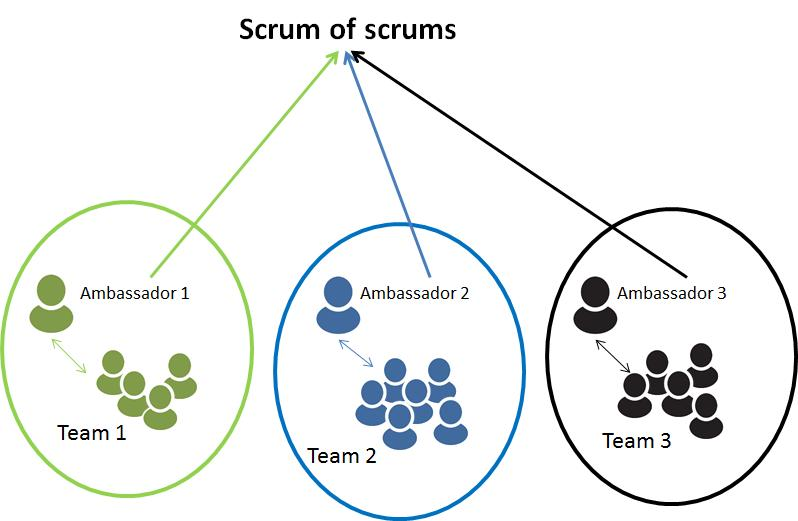
\includegraphics[width=0.75\textwidth]{figures/ScrumofScrum.png}
\caption{The structure of Scrum of Scrum. Figure from \cite{ScrumofScrumfigure}.}
\label{fig:ScrumofScrum}
\end{figure}

Every group will perform a daily Scrum individually, and the multi-group will perform a Scrum meeting answering the same questions as one would at daily Scrum but instead it is just the ambassadors from each group at this Scrum meeting, whom then speak on the group's behalf.
According to MountainGoatSoftware it is not necessary to have every day, and many organisations have them two to three times a week instead\footnote{\url{https://www.mountaingoatsoftware.com/agile/Scrum/team}}.
For the GIRAF project 2016, we have chosen to have one weekly Scrum every Wednesday instead.
The reasoning for this is that, the reports last year mentioned that two meetings a week was unnecessary, and while many organisations might have two to three a week, these organisations do not have courses to attend to, which also require a lot of time.
As the Scrum of Scrum meetings are held weekly the questions asked at these meeting change to asking: \enquote{...since last we met?} etc.
There are 4 other meetings than the weekly Scrum of Scrums specified for the multi--project by the Scrum Master:

\begin{description}
	\item[Sprint Planning] \hfill \\
	This meeting is held at the start of a sprint.
	In this meeting the groups can take tasks from the product backlog which they are interested in.
	The meeting is conducted by the Scrum Master which will introduce each user story in descending prioritised order.
	Each group can ask for a user story, if multiple groups ask for them, then they should argue why they should have the task until an agreement is reached.
	The result of this meeting is each group having user stories on their own sprint backlog, for them to complete during the coming sprint.
	\item[Sprint Retrospective] \hfill \\
	In the Sprint Retrospective the multi--project groups discuss the development process, with the purpose of reviewing and improving it.
	Here the groups can bring up any issues with the process in order to improve upon the process of the project.
	\item[Sprint Review] \hfill \\
	The customers attend the sprint review meeting so we can show them the progress of the applications, to gain valuable feedback, to create new tasks, and to help prioritise the tasks.
	\item[Presentations] \hfill \\
	This type of presentation is used to distribute information for relevant parties, i.e. a tour of Phabricator (will be described later).
	This is typically a presentation followed by questions from the attending parties.
	These meetings are less formal than the others and are only scheduled when needed.
\end{description}

Each sprint will be approximately 3 weeks, which gives time for approximately 4 sprints throughout the project.
At the start of each sprint the sprint planning meeting is held, afterwards the groups will estimate their chosen tasks.
When the sprint is over the sprint retrospective it held, and finally the sprint review.
The last two meetings might interchange, depending on the availability of the customers.
All the groups of the multi--project have agreed to use Scrum internally.

The Scrum master of the multi--project is group SW613F16, and they are the ones to make sure the other groups of the project adhere to the specified process.
The Scrum master is one of many areas of responsibility given to the groups this semester, which will be further explained in the next section.

\subsubsection*{Areas of Responsibility}
Every group of this years multi--project have an area of responsibility.
These responsibilities differ much in terms of amount of work, yet they are all important.
The different areas of responsibility are as follows:

\begin{description}
	\item[Server and Database] \hfill \\
	This area consists of maintaining the server and the database, including migrations and other maintenance and support tasks. They are essentially an internal IT service for the rest of the project. This area is covered by two groups: SW611F16, and SW616F16.
	\item[Social and Google Analytics] \hfill \\
	It is important that the groups of the multi--project know each other, and that they are all friendly with each other.
	This will make it easier for people to ask for help and work together.
	Google Analytics is a tool which help analyze and keep statistics of many things, such as how customer's find your application, or sending bug reports to the developers.
	The groups responsible for this is group SW612F16
	\item[Scrum Master] \hfill \\
	As mentioned earlier the Scrum master of the multi--project is group SW613F16
	\item[Product Owner and Security] \hfill \\
	The product owner of the multi--project is group SW614F16, they also have the areas of security, which means they will investigate any security measurements that are required for an application to be used by Aalborg municipality.
    These will henceforth be referred to as \textit{PO}.
	\item[Unit and Integration Tests] \hfill \\
	This area of responsibility involves making a guide for the multi--project such that the other groups can easily write new unit tests for their tasks.
	They also have to verify that the tests made by groups are thorough enough.
	The group responsible for this is group SW615F16.
	\item[Graphics and Sound] \hfill \\
	The GIRAF Application Suite needs graphic icons, and may also require sound for the games in the application.
	The group responsible for this is group SW617F16
	\item[Documentation and Wiki] \hfill \\
	This area requires establishing a standard of how documentation is done in the code, and responsible for the Wiki of the GIRAF project. We group SW618F16 are responsible for this areas.
	\item[Usability Tests] \hfill \\
	Performing usability tests on potential customers or with the customers themselves is important in order to know if the changes are working as intended, and to spot potential problems with the application. The group responsible for this is group SW619F16.
\end{description}

\section{Development and Organisational Tools}
Previously the project have used the project management tool Redmine.
However an opinion that is mostly consistent throughout all the papers from the previous semester is that Redmine should be replaced as it, according to last years students, is not a good tool.
Redmine offers tools for communication, calendars, documentation, issue tracking, a Wiki and more.
The primary issue with Redmine according to last years students refer to its lackluster communication solution.
As this is a problem stated throughout a majority of the papers the web application Slack is used as the communication tool between the groups involved in development.
Furthermore it was decided at the initial meeting to replace Redmine, with another software development tool: Phabricator, an open source, software development and project management platform. 
As Phabricator is still an unfamiliar tool issues may arise, however from the initial overview it seems to be geared towards agile development with applications specific to user stories and backlog tracking.
The workflow established for Phabricator is also very geared towards code review and documentation, something the groups agree seems very lackluster and should have more focus this semester\footnote{For more information about Phabricator visit their website at \url{http://phabricator.org/}}.
Lastly with Scrum meetings happening on a weekly basis a shared Google Docs folder contains all agendas and summaries from meetings.
Furthermore, while there is a primary rapporteur for each meeting, Google Docs allows everyone to pitch in for both the agenda and the summary which in turn means that if someone is not satisfied with the information in the summary, they can also add more information in real-time.

\subsection*{Gradle}\label{subsec:gradle}
In order to automate and introduce similar workflow when building the different parts of the GIRAF project, a build automation system is integrated into all parts of the GIRAF project --- \textbf{Gradle}\footnote{\url{http://www.gradle.org/}}.
Gradle is open source and builds upon the strengths and concepts of older build systems, e.g. Apache Ant\footnote{\url{http://ant.apache.org/}} and Apache Maven\footnote{\url{https://maven.apache.org/}}.
Moreover Gradle's syntax for project configurations is based on the JVM scripting language Groovy\footnote{\url{http://groovy-lang.org/}}.
Gradle is intended to be used in large projects and multi-part projects which contains numerous dependencies.
The tool determines which parts of the project already is up-to-date; this ensures that tasks dependent upon said parts does not need to be run again to build the entire project. 

By nature Gradle is plug-in focused, which enables it to be tailored to almost any type of build automation.
The main build configuration file of a project using Gradle is named \texttt{build.gradle}, and it contains information about dependencies, versions of said dependencies, and any tasks that are relevant for the given project.
                                       
Alternatives to using Gradle as build automation system are for example the aforementioned Maven and Ant tools, however these tools are dependent on writing build scripts in XML which is a markup language not suited for implementing logic into the automation process.
Furthermore Google recommends using Gradle and provides resources such as guides\footnote{\url{http://tools.android.com/tech-docs/new-build-system/user-guide}} and plug-ins for automating Android application builds using Gradle.

\subsection*{Workflow}
In this section we introduce the workflow for collaboration in the Giraf project, under Scrum of Scrum. 
Groups claim user stories for their sprint backlog at the sprint planning meeting, but it is possible to remove or claim more user stories during the sprint if needed. 
This is modeled in the \myref{fig:workflow}, the model also reveals that tasks are claimed prior to estimation.
The ability to remove or claim more user stories is a necessity as not only due to when estimation commences, but also because it is not possible to make exact estimates every time; although it is preferebly that it does not happen too often, such that groups are still generally aware of the tasks that will be completed for a given sprint.
Furthermore by claiming a task outside of the sprint planning meeting there will be no chance to discuss how it could be solved in general, making them harder to estimate and less concrete.
\myref{s1retro} explains how the multiproject reduces the impact of this weakness after the first sprint.

\bigskip 
\noindent
The remainder of the steps in \myref{fig:workflow} can be kept within the group, although review can be done by anyone not directly involved designing a proposed solution to a user story.
We have chosen to include a code review process in this years Giraf project. 
The reason for this is to increase the quality of the code, and its documentation, such as comments and javadocs. 
This can reduce the speed at which code is introduced, but we have deemed it reasonable due to a lot of the code current is hard to understand, and poorly documented. 
Code submitted to code review is called a diff, since it is the difference introduced by these changes relative to the current version. 
The person submitting code to review is responsible for finding suitable reviewers.
Typically one or more people with experience in the application or people who have done similar changes to other applications are asked to review.
A person can refuse to review a diff if they think they are not suited to review it, or the do not have time. 
A review is over once the one submitting the code for review is confident that what they have made is of a certain quality.
This quality is hard to define, and is subjective.
It should be noted that not all changes to the source code repositories strictly must go though the code review process.
Small insignificant changes, such as correcting spelling, or small graphical bug fixes can be pushed directly. 

\begin{figure}[H]
	\centering
	\begin{tikzpicture}[node distance = 0.5cm, auto]
	    \footnotesize
	    \node[wideblock]
	            (task) at (0,0)
	            {User story is introduced on Phabricator without a priority, either by a developer or the customer};
	        
	    \node[wideblock, below = of task]
	            (triage) {The PO of the multi-project give the user story a priority or discard it};
	            
	    \node[wideblock, below = of triage]
	            (planning) {User story is claimed by a project group on Phabricator};
	            
	    \node[wideblock, below = of planning]
	            (estimate) {The User Story is estimated by the project group};
	            
	    \node[wideblock, below = of estimate]
	            (branch) {A branch is created in git repository involving the user story, which uses the id of the user story};
	    
	    \node[wideblock, below = of branch]
	            (work) {The user story is completed and is ready for review, so a diff is created on Phabricator};
	            
	    \node[wideblock, below = of work]
	            (review) {A reviewer is chosen for the user story, and he/she reviews the diff and check if the user story is completed.};

	    \node[decision, below = of review]
	            (ready) {Changes?};

	    \node[wideblock, below = of ready]
	            (land) {The diff is applied to the master branch and the task is marked as completed on Phabricator};
	            
	    \path[line] (task) -- (triage);
	    \path[line] (triage) -- (planning);
	    \path[line] (planning) -- (estimate);
	    \path[line] (estimate) -- (branch);
	    \path[line] (branch) -- (work);
	    \path[line] (work) -- (review);
	    \path[line] (review) -- (ready);
	    \node[draw=none, right of = ready, node distance = 6.5cm] (cornerthree){};
	    \draw[-] (ready) -- node {yes} (cornerthree.center);
	    \path[line] (cornerthree.center) |- (work);
	    \path[line] (ready) -- node {no} (land);
	    
	\end{tikzpicture}
	\caption{Simplified workflow for the Giraf multi-project.}
	\label{fig:workflow}
\end{figure}


